\newif\ifvimbug
\vimbugfalse

\ifvimbug
\begin{document}
\fi

\exercise{Neural Networks}
In this exercise, you will use the dataset \texttt{mnist\_small}, divided into four files.

\begin{questions}

%----------------------------------------------

\begin{question}{Multi-layer Perceptron}{25}
Implement a neural network with one hidden layer and train it using backpropagation on the provided dataset. Choose your loss function, activation function and optimizer, briefly explaining your choices. You can use off-the-shelf optimizers, loss and activation functions, but you have to write the network structure and the backpropagation algorithm by yourself. You are also free to choose a suitable number of neurons for the hidden layer.

Plot the error during the training process against the number of iterations and attach snippets of your code. 


\begin{answer}
	As loss funtion, we use the mean squared error $\frac{1}{N }\sum_{n=1}^N y_{in,n} - y_{predict,n}$. For the activation function of the first layer, the sigmoid function $\varphi_1 = \frac{1}{1+e^{-Z}}$ is used, the activation function of the output layer is linear, $\varphi_2 = WX$, where $X$ is the matrix of all input vectors and Z the weighted and summed outputs of the hidden layer. As an optimizer, we use a simple gradient descent alogrithm
	
\lstinputlisting[language=Python, firstline=27, lastline=60]{../Code/4.2.py}
\end{answer}

The chosen number of hidden neurons is 10, the learning rate is set to 0.001 with 1000 iterations.

\centering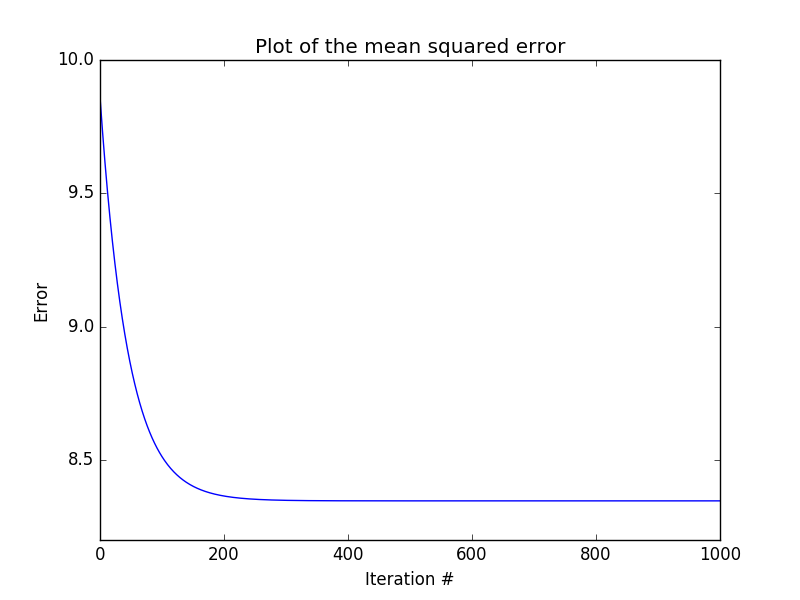
\includegraphics[width=0.7\linewidth]{4-1.png}



\end{question}

%----------------------------------------------

\begin{question}[bonus]{Deep Learning}{15}
In recent years, deep neural networks have become one of the most used tools in machine learning. 
Highlight the qualitative differences between classical neural networks and deep networks. Which limitations of classical NN does deep learning overcome?
Give an intuition of the innovations introduced in deep learning compared to traditional NN.
(Hint: have a look \href{http://arxiv.org/abs/1206.5538}{at this paper} and \href{https://plus.google.com/100849856540000067209/posts/9BDtGwCDL7D}{at this Google+ discussion}.)

\begin{answer}
\emph{Deep networks} differ from classical neural networks in their number of hidden layers. Classical neural networks commonly have one or two hidden layers and are used for supervised learning only. However, deep networks have way more hidden layers and can be trained in an supervised and unsupervised way in order to cope with supervised and unsupervised learning problems.\\

The limitations of classical neural networks are their low amount of hidden layers, which leads to  linear dependencies of the bottom layer from the layers above. This directly limits what kind of problems the neural network can learn. However, the addition of more layers vastly increases the quality of the learning algorithm. As each hidden unit is connected to many other hidden units below, each hidden layer can be seen as a non-linear combination of the layers below. The additional optimization transforms the layers into optimally weighted, non-linear combinations of the layers below. Adding a decrease of dimensionality to each layer, as each sequential hidden layer has less units than the one below, results in a lower dimensional projection from layer to layer. In summation this results in a non-linear, optimally weighted, lower dimensional projection in each subsequent layer of the deep network.

Furthermore, when using machine learning appraoches like SVM, one has to invest a big deal into (hand-crafted) feature extraction for the given problem. As the automated process of deep learning already includes a high-level feature extraction this is not neccessary and taken care of by the deep learning algorithm.
\end{answer}

\end{question}

%----------------------------------------------

\end{questions}
